\documentclass[12pt, a4paper]{article}
\usepackage[utf8]{inputenc}
\usepackage{ragged2e}

\usepackage{graphicx, geometry, hyperref, wrapfig, amsmath, subcaption, setspace}
\usepackage[dvipsnames]{xcolor}

\definecolor{silver}{RGB}{200,200,200}
\hypersetup{colorlinks=true, linkcolor=RoyalBlue, urlcolor=RoyalBlue}

 \geometry{
 a4paper,
 total={175mm,257mm},
 left=20mm,
 top=15mm,
 }

\usepackage{xcolor} % for defining colour
\usepackage{titlesec} % for customizing sections

% \usepackage{times}        % Use Times New Roman font
% \usepackage{helvet}       % Use Helvetica font
\usepackage{palatino}

\usepackage[T1]{fontenc}

\setlength\parindent{0pt}

% %%%%%%%%%%%%%%%%%%%%%%%%%%%%%%%%%%%%%%%%%%%%%%%%%%%%%%%%%%%%%%
\titleformat{\section}
{\color{UM_DarkBlue}\normalfont\large\bfseries}
{\color{UM_DarkBlue}\thesection}{1em}{}

%%%%%%%%%%%%%%%%%%%%%%%%%%%%%%%%%%%%%%%%%%%%%%%%%%%%%%%%%%%%%%%
\definecolor{UM_Brown}{HTML}{3D190D}
\definecolor{UM_DarkBlue}{HTML}{2264B0}
\definecolor{UM_LightBlue}{HTML}{1CA9E1}
\definecolor{UM_Orange}{HTML}{fEB415}

%%%%%%%%%%%%%%%%%%%%%%%%%%%%%%%%%%%%%%%%%%%%%%%%%%%%%%%%%%%%%%%%

\newcommand{\eg}{{\it e.g.}}
\newcommand{\ie}{{\it i.e.}}

% %%%%%%%%%%%%%%%%%%%%%%%%%%%%%%%%%%%%%%%%%%%%%%%%%%%%%%%%%%%%%%
% \hypersetup{
%     draft=false,
%     final=true,
%     colorlinks=true,
%     citecolor=UM_DarkBlue,
%     anchorcolor=yellow,
%     linkcolor=UM_DarkBlue,
%     urlcolor=UM_DarkBlue,
%     filecolor=green,      
%     pdfpagemode=FullScreen,
%     bookmarksopen=false
%     }
\usepackage{amsmath,amsfonts,amssymb,bm}

%%%%%%%%%%%%%%%%%%%%%%%%%%%%%%%%%%%%%%%%%%%%%%%%%%%%%%%%%%%%%
% Sets and Notations
\newcommand{\reals}{\mathbb{R}}
\newcommand{\integers}{\mathbb{Z}}

%%%%%%%%%%%%%%%%%%%%%%%%%%%%%%%%%%%%%%%%%%%%%%%%%%%%%%%%%%%%%
% Vectors and Matrices
% \renewcommand{\vec}[1]{\bm{\mathrm{#1}}}
\newcommand{\dotp}{\,\boldsymbol{\cdot}\,}
\newcommand{\grad}[1]{\vec{\nabla}#1}
\renewcommand{\div}[1]{\vec{\nabla}\!\dotp\!\vec{#1}}
\newcommand{\curl}[1]{\vec{\nabla}\!\times\!\vec{#1}}



%%%%%%%%%%%%%%%%%%%%%%%%%%%%%%%%%%%%%%%%%%%%%%%%%%%%%%%%%%%%%
% Derivatives
\newcommand{\dv}[2]{\frac{d#1}{d#2}}
\newcommand{\ndv}[3][2]{\frac{d^{\,#1}#2}{d#3^{\,#1}}}

\newcommand{\pdv}[2]{\frac{\partial#1}{\partial#2}}
\newcommand{\npdv}[3][2]{\frac{\partial^{\,#1}#2}{\partial#3^{#1}}}
 
\title{OWO-GAship}
\author{Anik Mandal}
\date{January 2025}
\pagenumbering{arabic}
\setstretch{1.4}

%====================================================================================================
\begin{document}


\begin{minipage}[t][][c]{0.1\textwidth}
    \begin{flushleft}
        
\includegraphics[height=2cm]{tex-resources/Ashoka Logo.png}
    \end{flushleft}
\end{minipage}
\begin{minipage}[t][][c]{0.85\textwidth}
    \begin{center}
        {\LARGE Oscillations, Wave and Optics}\\ \vspace{0.5em}
        \textsc{(Spring 2025)}\\
        \vspace{1em}
        \textbf{\Large FINAL TERM RESITTING} \\
    \end{center}
\end{minipage}
\vspace{20pt}\\
\rule[0em]{\textwidth}{0.75pt}

\flushleft{Date: \hspace{1in}}\hfill
\fbox{\textbf{\large 
Time: \hspace{1in}}}\hfill
\textbf{\large 
Mark: 100}\\

\textbf{Instructions}:
\begin{itemize}
    \item Write physics arguments and definitions clearly while arriving at the mathematical proofs.
    Unclear statements, mathematical proofs will not be considered. 
    \item You are not allowed to use any kind of study materials or books during the exam.
    (Only a scientific calculator is allowed if required)
    \item Answer all 4 problems.
\end{itemize}
\begin{center}
    \textbf{All the best!!!}
\end{center}
\rule[0em]{\textwidth}{1.75pt}
\vspace{-1cm}

%====================================================================================================
%====================================================================================================
\justifying

%#######################################
\section*{Problem-1 \hfill \textbf{[25]}}
\noindent
\textbf{(1)} A body hung at the end of a light vertical spring stretches the spring statically to 
twice its original length. The system can be set into motion either as a simple pendulum or as a 
mass-spring oscillator. Determine the ratio between the periods of these motions. (In the pendulum 
mode of motion, assume the length of the spring to be constant.)\hfill\textbf{5}


\begin{figure}[h]
    \centering
    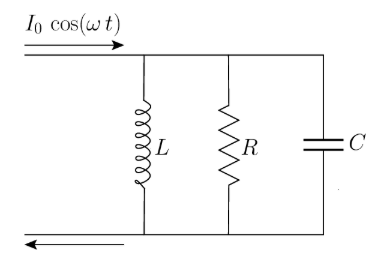
\includegraphics[scale=0.5]{figs/LCR-circuit.png}
    \caption{}
    \label{fig:LCR-circuit}
\end{figure}

\noindent
\textbf{(2)} What are the resonant angular frequency and quality factor of the circuit shown in 
Figure-\ref{fig:LCR-circuit}? What is the average power absorbed at resonance?\hfill\textbf{5+5}

\noindent
\textbf{(3)} Demonstrate that in the limit $\nu \rightarrow 2\omega_0$ the solution to the damped 
harmonic oscillator equation becomes
\begin{equation*}
    x(t) = (x_0 + [v_0+ \omega_0 x_0]t){e}^{-\omega_0 t}
\end{equation*}
where $x_0=x(0)$ and $v_0=\dot{x}(0)$.\hfill\textbf{5}

\noindent
\textbf{(4)} Determine the fourier coefficients and express the given periodic function in terms of 
fourier series. \hfill\textbf{5}
\[ f(x) =
\begin{cases} 
-x, & \text{for } -\pi< x < 0 \\
0, & \text{for } 0\leq x <\pi
\end{cases}
\] 

%#######################################
\section*{Problem-2 \hfill \textbf{[30]}}

\noindent
\textbf{(1)} Consider a mass-spring system of the general form shown in Figure-\ref{fig:Coupled-Osc} 
in which the springs all have spring constant $k$, and the left and right masses are of mass $m$ 
and $m'$, respectively. Find the normal frequencies and normal modes in terms of $\omega_0=\sqrt{k/m}$
and $\alpha=m'/m$. \hfill\textbf{10}

\begin{figure}[h]
    \centering
    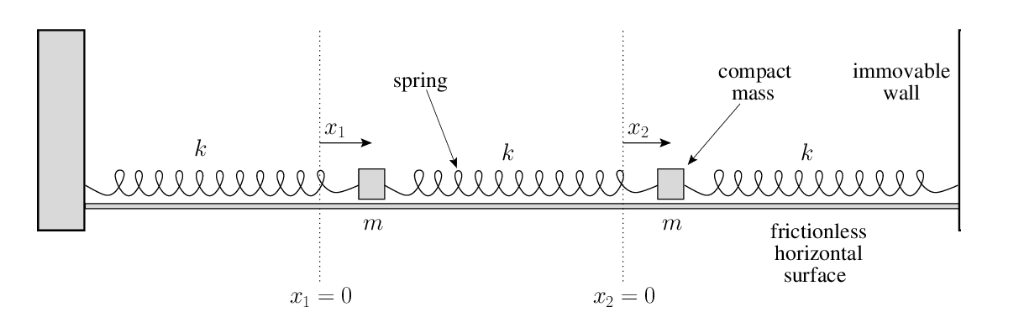
\includegraphics[scale=0.3]{figs/Coupled-Osc.png}
    \caption{}
    \label{fig:Coupled-Osc}
\end{figure} 



\noindent
\textbf{(2)} A simple model of an ionic crystal consists of a linear array of a great many 
equally-spaced  atoms of same masses $m$. The masses are connected by alternating chemical 
bonds that are modeled as springs of spring constants $K_1$ and $K_2$ ($K_2$ > $K_1$) as shown 
in the figure-\ref{fig:Alternating_chain}. \hfill\textbf{10 + 5}
\begin{figure}[h]
    \centering
    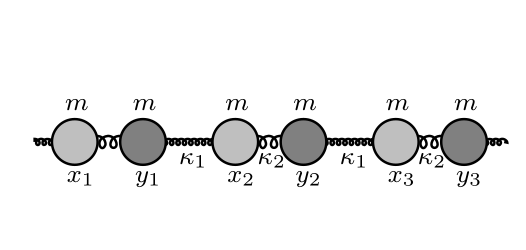
\includegraphics[scale=0.4]{figs/Alternating_chain.png}
    \caption{}
    \label{fig:Alternating_chain}
\end{figure} 

\textbf{i.} Show that the frequencies of the system's longitudinal modes of vibration either lie in 
the band 0 to $(2K_1/m)^{1/2}$ or in the band $(2K_2/m)^{1/2}$ to $[2(K_1 + K_2)/m)]^{1/2}$.

\textbf{ii.} Show that, in the long-wavelength limit, modes whose frequencies lie in the lower band
are such that  neighboring atomics move in the same direction, whereas modes whose frequencies lie 
in the upper band are such that neighboring atoms move in opposite directions. 


\noindent
\textbf{(3)} Consider a uniform string of length $l$, tension $T$, and mass per unit length $\rho$ 
that is stretched between two immovable walls. Show that the total energy of the string, which is 
the sum of its kinetic and potential energies, is
\begin{equation*}
    E = \frac{1}{2}\int_0^l[\rho(\frac{\partial y}{\partial t})^2
+ T(\frac{\partial y}{\partial x})^2] dx,
\end{equation*}

where $y(x,t)$ is the string's (relatively small) transverse displacement. \hfill \textbf{5}

%#######################################
\section*{Problem-3 \hfill \textbf{[15]}}

\noindent
\textbf{(1)} Two co-axial transmission lines of impedances $Z_1$ and $Z_2$ are connected as indicated in 
Figure-\ref{fig:Transmission_with_resistor}. That is, the outer conductors are continuous, whereas the inner
wires are connected to either side of a resistor of resistance $R_L$. The length of the resistor is 
negligible compared to the wavelengths of the signals propagating down the line. Suppose that $Z_1>Z_2$. 
\begin{figure}[h]
    \centering
    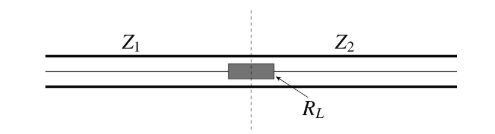
\includegraphics[scale=0.4]{figs/Transmission_with_resistor.png}
    \caption{}
    \label{fig:Transmission_with_resistor}
\end{figure}

\textbf{i.} Suppose, further, that a signal is incident on the junction along the line whose impedance is $Z_1$.
Show that the coefficients of reflection and transmission are
\begin{equation*}
    R = (\frac{R_L-Z_1+Z_2}{R_L+Z_1+Z_2})^2,
    T = \frac{4\,Z_1\,Z_1}{(R_L+Z_1+Z_2)^2},
\end{equation*}
	   
respectively. \hfill\textbf{8}

\textbf{ii.} Hence, deduce that the choice

\begin{equation*}
    R_L= Z_1-Z_2
\end{equation*}
suppresses reflection at the junction. Demonstrate that, in this case, the fraction of the incident 
power absorbed by the resistor is \hfill\textbf{2+5}
\begin{equation*}
    A=1-\frac{Z_2}{Z_1}
\end{equation*}

%#######################################
\section*{Problem-4 \hfill \textbf{[30]}}

\noindent
\textbf{(1)} Starting from the basic Maxwell's equations in electrodynamics, derive the Fresnel 
relations for obliquely incident of EM wave on a plane interface between two dielectric media.
Consider the polarization state in which electric components of the incident, reflected, and 
refracted waves are all parallel to the interface. \hfill\textbf{10}

\noindent
\textbf{(2)} Show that a light-ray entering a planar transparent plate of thickness $d$ and 
refractive index $n$ emerges parallel to its original direction. Show that the lateral displacement 
of the ray is
\begin{equation*}
    s = \frac{d\,\sin(\theta_1-\theta_2)}{\cos\theta_2}
\end{equation*}
where $\theta_1$ and $\theta_2$ are the angles of incidence and refraction, respectively, at the 
front side of the plate. \hfill\textbf{5}

\noindent
\textbf{(3)} Estimate how large the lens of a camera carried by an artificial satellite orbiting the 
Earth at an altitude of 150 miles would have to be in order to resolve features on the Earth's 
surface a foot in diameter. \hfill\textbf{5}
 
\noindent
\textbf{(4)} Derive the expression for the far-field interference pattern($\mathcal{I}(\theta)$), 
created by a monocromatic light of wavelength $\lambda$ when it encounters $10$ narrow identical 
slit with equal spacing($d$), running parallel to the $y$-axis. \hfill\textbf{10}

\end{document}